\documentclass{school}

\subject{Angewandte Mathematik}
\title{Zahlentheorie und Matrizenrechnung}
\subtitle{Jahrgang 4 \-- Semester 2 \-- Schularbeit 4}

\author{Markus Reichl}

\begin{document}

\maketitle
\tableofcontents

\newpage
\section{Zahlentheorie}
\subsection{Einführung}
Es sei $x$ mit $x \in \mathbb{N}$ eine beliebige natürliche Zahl mit $n \ge 2$ mit $n \in \mathbb{N}$.
Dann gelte: $$x = q*n + r$$
\begin{center}
    \begin{tabular}{l l}
        n & \dots Modul \\
        q & \dots $int(x/n), q \in \mathbb{N}$\\
        r & \dots Nicht negativer Rest
    \end{tabular}
\end{center}
Die Kurzschreibweise zur Berechnung von $r$ lautet
$$r = x ~\mod~ n \quad \widehat{=} \quad r = x - n * q$$
Für Modulo $n$ existieren genau $n$ Restklassen
$$\{0, 1, 2, \ldots, n - 1\}$$

\subsubsection{Kongruenz}
2 natürliche Zahlen sind kongruent, wenn diese denselben, nicht negativen, Rest haben.
$$a \equiv b \to a ~\%~ n = b ~\%~ n$$

\paragraph{Regeln}~\\
Kongruenzen können multipliziert werden
$$a \equiv b \text{ und } c \equiv d \to a * c \equiv b * d$$
Kongruenzen können zu gleichen Potenzen erhöht werden
$$a \equiv b \to a^k \equiv b^k$$

\subsection{Square and Multiply}
Bei dieser Methode wird der Exponent in 2er Potenzen zerlegt.
\paragraph{Bsp.: $9^{23} ~\mod~ 7$}
$$9^{23} = 9^{16} * 9^{4} * 9^{2} * 9$$
$$9 \equiv 2$$
Die Potenzregel kann angewandt werden um die weiteren Potenzen zu bestimmen.
$$9^2 \equiv 2^2 = 4$$
$$9^4 \equiv 2^4 = 16 \equiv 2$$
$$9^{16} \equiv 2^4 = 16 \equiv 2$$
Anhand der Faktorregel können nun die Kongruenzen als Faktoren eingesetzt werden.
$$9^{23} \equiv 2 * 4 * 2 * 2 = 32$$
$$9^{23} \equiv 4$$

\subsection{Kodierung und Dekodierung}
\begin{tabular}{l l l}
    \textbf{Symmetrisch} & Gleicher Schlüssel für Ver- und Entschlüsselung & Bsp.: Cäsar \\
    \textbf{Asymmetrisch} & Verschiedene Schlüssel für Ver- und Entschlüsselung & Bsp.: RSA
\end{tabular}

\subsubsection{Cäsar}
\begin{center}
    \begin{tabular}{r c c c c c l}
        & B & R & A & V & O &\\
        & $\downarrow \uparrow$ & $\downarrow \uparrow$ & $\downarrow \uparrow$ & $\downarrow \uparrow$ & $\downarrow \uparrow$ &\\
        & 02 & 18 & 01 & 22 & 15 &\\
        $+ (c ~\%~ 27)$ & $\downarrow \uparrow$ & $\downarrow \uparrow$ & $\downarrow \uparrow$ & $\downarrow \uparrow$ & $\downarrow \uparrow$ & $+ 27 - (c ~\%~ 27)$\\
        & 10 & 26 & 11 & 03 & 23 &\\
        & $\downarrow \uparrow$ & $\downarrow \uparrow$ & $\downarrow \uparrow$ & $\downarrow \uparrow$ & $\downarrow \uparrow$ &\\
        & J & Z & I & C & W &
    \end{tabular}
\end{center}

\subsubsection{RSA}
\begin{enumerate}
    \item A wählt 2 Primzahlen $p, q$ als \textbf{Private Key}
    \item A wählt eine Zahl $e$ (Encrypt), welche teilerfremd\footnote{Zwei natürliche Zahlen und sind teilerfremd, wenn es keine natürliche Zahl außer Eins gibt, welche beide Zahlen teilt.} zu $(p-1)*(q-1)$ ist
    \item A veröffentlicht seinen \textbf{Public Key} bestehend aus der Zahl $e$ und dem Produkt $n$ aus $$n = p * q$$
    \item B möchte eine Nachricht an A senden und wandelt diese in eine Zahl um. Diese Zahl wird in $x$ gleich lange Blöcke zerlegt. Die resultierende Nachricht $y$ lautet $$y = x^e ~\mod~ n$$
    \item A berechnet den Private Key $d$ (Decrypt) aus $$d = \frac{1 + k(p-1)(q-1)}{e} \quad\quad k \in \mathbb{N}$$
    \item A erhält die Nachricht $y$ und ermittelt $x$ aus $$x = y^d ~\mod~ n$$
\end{enumerate}

\paragraph{Bsp.: ``BRAVO''}
\begin{enumerate}
    \item B möchte die Nachricht ``BRAVO'' an A senden und findet dafür den Public Key $$n = 1147 ~\text{mit}~ e = 29$$
    \item Zur Verschlüsselung wird die Nachricht in Zahlen umgewandelt und in gleich lange Blöcke unterteilt. Der letzte Block wird an der rechten Seite mit 0 aufgefüllt.
    \begin{center}
        \begin{tabular}{c c c c c}
            B & R & A & V & O\\
            $\downarrow$ & $\downarrow$ & $\downarrow$ & $\downarrow$ & $\downarrow $\\
            02 & 18 & 01 & 22 & 15\\
            $\downarrow$ & $\downarrow$ & $\downarrow$ & $\downarrow$ & $\swarrow $\\
            021 & 801 & 221 & 500 &
        \end{tabular}
    \end{center}

    \item Nun werden die einzelnen Blöcke anhand des Public Keys kodiert. Diesmal werden zu kurze Blöcke an der linken Seite mit 0 aufgefüllt.
    $$y_n = {x_n}^e ~\mod~ n$$
    \begin{center}
        \begin{tabular}{c c c c}
            021 & 801 & 221 & 500\\
            $\downarrow$ & $\downarrow$ & $\downarrow$ & $\downarrow$\\
            003 & 533 & 628 & 535
        \end{tabular}
    \end{center}
    \item A empfängt die Nachricht und nutzt seinen Private Key $p = 31, q = 37$ und findet den Schlüssel $d$ aus
    $$d = \frac{1 + k(p-1)(q-1)}{e}$$~\\
    $k$ wird dabei in natürlichen Schritten gesteigert, bis $d$ ganzzahlig ist. Hier bei $k = 4$.
    $$d = \frac{1 + 4 * 30 * 36}{29} = 149$$
    \item A erhält nun die Nachricht $x$ aus $$x_n = {y_n}^d ~\mod~ n$$
    Zu kurze Blöcke werden von links aufgefüllt.
    \begin{center}
        \begin{tabular}{c c c c c c}
            003 & 533 & 628 & 535 & &\\
            $\downarrow$ & $\downarrow$ & $\downarrow$ & $\downarrow$ & &\\
            021 & 801 & 221 & 500 & &\\
            $\downarrow$ & $\downarrow$ & $\downarrow$ & $\downarrow$ & $\searrow$ &\\
            02 & 18 & 01 & 22 & 15 & 00\\
            $\downarrow$ & $\downarrow$ & $\downarrow$ & $\downarrow$ & $\downarrow$ & $\downarrow$\\
            B & R & A & V & O & \_
        \end{tabular}
    \end{center}
\end{enumerate}

\section{Matrizenrechnung}
\subsection{Grundlagen Vektoren}
Vektoren sind gerichtete Größen, definiert durch ihren Betrag und ihre Länge.\\
Sie geben also keine Punkte, sondern eine Richtung an.
$$\vec{a} = \binom{a_x}{a_y}$$
\begin{center}
    \begin{tabular}{l l}
        $a_x$ & \dots Schaft\\
        $a_y$ & \dots Spitze\\
    \end{tabular}
\end{center}

\begin{figure}[hh]
    \centering
    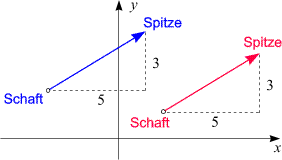
\includegraphics[width=0.4\textwidth]{vektor1.png}
    \caption[http://www.mathe-online.at/mathint/vect1/grafiken/vektor1.gif]{Vektoren im $\mathbb{R}^2$}
    \label{fig:vektor}
\end{figure}

\subsubsection{Typen}
\paragraph{Einheitsvektor}
Vektoren mit der Länge 1 werden als Einheitsvektoren oder auch normierte Vektoren bezeichnet.
$$\vec{a_E} = \frac{\vec{a}}{|\vec{a}|}$$

\paragraph{Inverser Vektor}
Ein Vektor ist invertiert wenn $\vec{a}$ und $-\vec{a}$ gleich lang aber entgegengesetzt gerichtet sind.
$$\vec{a} = \binom{a_x}{a_y} \to -\vec{a} = \binom{-a_x}{-a_y}$$

\paragraph{Ortsvektor}
Ein Vektor vom Ursprung $O(0|0)$ zu einem bestimmten Punkt.
$$\overrightarrow{OP} = \binom{P_x}{P_y}$$

\paragraph{Normalvektor}
Zwei Vektoren sind aufeinander normal, wenn deren x und y-Koordinaten vertauscht sind und ein Vorzeichen geändert wird.
$$\vec{a} \perp \vec{b} ~\text{wenn}~ \vec{a} = \binom{a_1}{a_2} ~\text{und}~ \vec{b} = \binom{-a_2}{a_1} ~\text{oder}~ \vec{b} = \binom{a_2}{-a_1}$$

\newpage
\subsubsection{Rechenregeln}
\paragraph{Betrag}
Die Länge eines Vektors ist als dessen Betrag definiert. Dieser kann über den Satz des Pythagoras hergeleitet werden.
$$|\vec{a}| = \sqrt{{a_x}^2 + {a_y}^2}$$

\paragraph{Addition und Subtraktion}
Vektoren werden addiert oder subtrahiert indem deren Elemente nach Zeile addiert bzw.\ subtrahiert werden.
$$\binom{a_x}{a_y} \pm \binom{b_x}{b_y} = \binom{a_x \pm b_x}{b_y \pm b_y}$$

\paragraph{Skalare Multiplikation}
Vektoren werden mit Zahlen multipliziert, indem jedes Element einzeln mit dem Faktor multipliziert wird.
$$\binom{a_x}{a_y} * b = \binom{a_x * b}{a_y * b}$$

\paragraph{Skalarprodukt zweier Vektoren}
Das Skalarprodukt zweier Vektoren ist von der Länge der Vektoren und dem eingeschlossenen Winkel abhängig.
$$\vec{a} * \vec{b} = |\vec{a}| * |\vec{b}| * \cos(\varphi)$$
$$\varphi = \sphericalangle(\vec{a}, \vec{a})$$
\begin{figure}[hh]
    \centering
    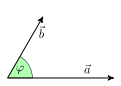
\includegraphics[width=0.2\textwidth]{skalar.png}
    \caption[https://de.wikipedia.org/wiki/Skalarprodukt\#/media/File:Dot-product-3.3.svg]{Skalarprodukt}
    \label{fig:skalar}
\end{figure}~\\
Berechnet wird dieses aus
$$\binom{a_x}{a_y} * \binom{b_x}{b_y} = a_x * b_x + a_y + b_y$$
Das Skalarprodukt zweier Vektoren ist genau dann 0, wenn gilt $cos(\varphi) = 0$\footnote{Dies ist sowohl bei 90, als auch bei 270 Grad der Fall}, oder der Betrag eines Vektors 0 ist. In diesem Fall sind die Vektoren zueinander orthogonal.

\newpage
\subsection{Grundlagen Matrizen}
Eine Matrix vom Typ ($m \times n$) ist ein Schema aus $m$ Zeilen und $n$ Spalten.
$$
A = \begin{pmatrix}
a_{11} & a_{12} & a_{13} & ... & a_{1n}\\
a_{21} & a_{22} & a_{23} & ... & a_{2n}\\
\vdots & \vdots & \vdots & & \vdots\\
a_{m1} & a_{m2} & a_{m3} & ... & a_{mn}
\end{pmatrix}
$$
\begin{center}
    \begin{tabular}{l l}
        $a_{mn}$ & \dots Element der Matrix \\
        $m$ & \dots Zeile\\
        $n$ & \dots Spalte
    \end{tabular}
\end{center}

\paragraph{Zeilenvektor}
Eine Matrix mit nur einer Zeile.
$$(1 \times 3) \to A\begin{pmatrix}1 & 2 & 3\end{pmatrix}$$

\paragraph{Spaltenvektor}
Eine Matrix mit nur einer Spalte.
$$(3 \times 1) \to A\begin{pmatrix}1\\2\\3\end{pmatrix}$$

\paragraph{Skalar}
Eine einzelne Zahl kann auch als eine Matrix mit einer Zeile und einer Spalte gesehen werden. Eine solche Matrix nennt man einen Skalar.
$$(1 \times 1) \to A = 1$$

\paragraph{Quadratische Matrix}
Die Anzahl der Zeilen ist gleich der Anzahl der Spalten ($m = n$).
$$(2 \times 2) \to A\begin{pmatrix}1 & 2\\1 & 2\end{pmatrix}$$

\paragraph{Diagonalmatrix}
Alle Elemente außerhalb der Hauptdiagonale sind gleich 0.
$$(3 \times 3) \to A\begin{pmatrix}1 & 0 & 0\\ 0 & 2 & 0\\ 0 & 0 & 3\end{pmatrix}$$

\paragraph{Einheitsmatrix}
Alle Elemente der Hauptdiagonale sind gleich 1 und jene außerhalb 0.
$$(3 \times 3) \to A\begin{pmatrix}1 & 0 & 0\\ 0 & 1 & 0\\ 0 & 0 & 1\end{pmatrix}$$

\paragraph{Transponierte Matrix}
Zeilen und Spalten einer Matrix werden vertauscht.\\
Dabei wird jede Zeile zu einer Spalte.
$$A\begin{pmatrix}1 & 2 & 3\\ 4 & 5 & 6\end{pmatrix} \to A^T\begin{pmatrix}1 & 4\\2 & 5 \\3 & 6\end{pmatrix}$$

\paragraph{Symmetrische Matrix}
Jede Diagonale einer Matrix enthält nur ein Element. Es gilt $A = A^T$.
$$(3 \times 3) \to A\begin{pmatrix}1 & 2 & 3\\ 2 & 1 & 2\\ 3 & 2 & 1\end{pmatrix}$$

\subsubsection{Rechenregeln}
\paragraph{Addition und Subtraktion}
Die Addition 2er Matrizen $A$ und $B$ ist nur dann definiert, wenn diese vom selben Typen sind ($A_m = B_m$ und $A_n = B_n$).
$$A + B = C \to A_{mn} \pm B_{mn} = C_{mn}$$
$$
A \begin{pmatrix}
a_{11} & a_{21}\\
a_{21} & a_{22}
\end{pmatrix} \pm
B \begin{pmatrix}
b_{11} & b_{21}\\
b_{21} & b_{22}
\end{pmatrix} =
C \begin{pmatrix}
a_{11} \pm b_{11} & a_{21} \pm b_{21}\\
a_{21} \pm b_{21} & a_{21} \pm b_{22}
\end{pmatrix}
$$

\paragraph{Skalare Multiplikation}
Jedes Element einer Matrix wird mit dem Faktor multipliziert.
$$
A \begin{pmatrix}
a_{11} & a_{21}\\
a_{21} & a_{22}
\end{pmatrix} * b =
C \begin{pmatrix}
b * a_{11} & b * a_{21}\\
b * a_{21} & b * a_{22}
\end{pmatrix}
$$

\newpage
\paragraph{Multiplikation von Matrizen}
$C$ ist als Produkt von $A * B$ nur dann definiert wenn gilt
$$A(m \times p) \quad \text{und} \quad B(p \times n)$$
Damit ist $C$ eine $(m \times n)$ Matrix definiert als
$$C_{mn} = \sum_{i = 1}^{p} a_{mi} * b_{in}$$
ACHTUNG! Die Multiplikation von Matrizen ist NICHT kommutativ!
$$A \cdot B \ne B \cdot A$$

\paragraph{Beispiel}
$$A\begin{pmatrix}
    1 & 2 & 3\\
    4 & 5 & 6\\
    7 & 8 & 9
\end{pmatrix}
B\begin{pmatrix}
    1 & 2\\
    3 & 4\\
    5 & 6
\end{pmatrix}
$$
~\\
Zur Berechnung der Matrix  $C = A \cdot B$ ist es sinnvoll, die Matrizen versetzt nebeneinander zu schreiben, diese Methode nennt man auch Falk'sches Schema.
\subparagraph{Falk'sches Schema}
\begin{center}
    \begin{tabular}{c c}
        \begin{tabular}{c c c c | c | c |}
            & & & & 1 & 2\\
            & & & B & 3 & 4\\
            & & $\cdot$ & & 5 & 6\\
            & A & & & $\downarrow$ & $\downarrow$ \\\hline
            1 & 2 & 3 & $\to$ & $c_{11}$ & $c_{12}$\\\hline
            4 & 5 & 6 & $\to$ & $c_{21}$ & $c_{22}$\\\hline
            7 & 8 & 9 & $\to$ & $c_{31}$ & $c_{32}$
        \end{tabular}
        &
        \begin{tabular}{l   }
            $c_{11} = 1 * 1 + 2 * 3 + 3 * 5 = 22$\\
            $c_{12} = 1 * 2 + 2 * 4 + 3 * 6 = 28$\\
            $c_{21} = 4 * 1 + 5 * 3 + 6 * 5 = 49$\\
            $c_{22} = 4 * 2 + 5 * 4 + 6 * 6 = 64$\\
            $c_{31} = 7 * 1 + 8 * 3 + 9 * 5 = 76$\\
            $c_{32} = 7 * 2 + 8 * 4 + 9 * 6 = 100$
        \end{tabular}
    \end{tabular}
\end{center}
$$A \begin{pmatrix}
    1 & 2 & 3\\
    4 & 5 & 6\\
    7 & 8 & 9
\end{pmatrix} \cdot
B \begin{pmatrix}
    1 & 2\\
    3 & 4\\
    5 & 6
\end{pmatrix} =
C \begin{pmatrix}
    22 & 28\\
    49 & 64\\
    76 & 100
\end{pmatrix}
$$

\newpage
\subsubsection{Determinanten}
\paragraph{Definition}
\begin{center}
`Eine Determinante ist eine Zahl, die einer quadratischen Matrix zugeordnet ist.
Man kann die Determinante jeder allgemeinen Matrix vom Typ $(m \times m)$ bestimmen``~\cite{determinante}
\end{center}

\paragraph{Eigenschaften}
\begin{itemize}
    \item Die Determinante einer Matrix $A$ ist gleich jener der transposierten Matrix $A^T$. $$|A| = |A^T|$$
    \item Der Wert einer Determinante ist unabhängig von der Entwicklungszeile / -spalte.
    \item Eine Determinante ist gleich Null, wenn einer der folgenden Fälle zutrifft:
    \begin{itemize}
        \item eine Zeile / Spalte besteht aus lauter Nullen
        \item zwei Zeilen / Spalten sind gleich
        \item eine Zeile / Spalte ist eine Linearkombination anderer Zeilen/Spalten
    \end{itemize}
    \item Vertauscht man eine gerade Anzahl an Zeilen / Spalten ändert sich das Vorzeichen der Determinante.
    \item Multipliziert man eine Zeile / Spalte mit einer Zahl, wird die Determinante ebenfalls multipliziert.
    \item Die Determinante des Produktes zweier Matrizen entspricht dem ihrer Determinanten. $$|A \cdot B| = |A| \cdot |B|$$
\end{itemize}

\newpage
\paragraph{Berechnung}
\subparagraph{$2 \times 2$ (Diagonalen)}
Die Determinante einer Matrix $2 \times 2$ entspricht dem Produkt der Hauptdiagonale abzüglich des Produktes der Nebendiagonale.
$$\begin{vmatrix}a & b\\c & d\end{vmatrix} = a * d - b * c$$
\subparagraph{$3 \times 3$ (Regel von Sarrus)}
Bei dieser Regel werden zu Beginn die ersten beiden Spalten noch einmal neben die Determinante geschrieben.
$$
\begin{vmatrix}
a & b & c\\
d & e & f\\
g & h & i
\end{vmatrix} \quad \to \quad
\begin{matrix}
a & b & c\\
d & e & f\\
g & h & i
\end{matrix}
\quad \vrule \quad
\begin{matrix}
a & b\\
d & e\\
g & h
\end{matrix}
$$
Jetzt bildet man die Produkte der Elemente der drei Diagonalen, welche von links oben nach rechts unten verlaufen.
Diese Produkte werden addiert.
$$a * e * i + b * f * g + c * d * h$$
Von dieser Menge werden nun die Produkte der Elemente der drei Diagonalen, welche von links unten nach rechts oben verlaufen, abgezogen.
$$- g * e * c - h * f * a - i * d * b$$
Die Formel zur Berechnung einer $3 \times 3$ Determinante lautet also wie folgt.
$$
\begin{vmatrix}
a & b & c\\
d & e & f\\
g & h & i
\end{vmatrix} = aei + bfg + cdh - gec - hfa - idb
$$

\newpage
\subsection{Gauß Algorithmus}
Ein lineares Gleichungssystem in $n$ Gleichungen und $n$ Unbekannten ist als Matrix genau dann eindeutig lesbar wenn $|A| \ne 0$ gilt.
\vspace{1 em}\\
Als Beispiel ist folgendes lineares Gleichungssystem in $3$ Gleichungen und $3$ Unbekannten gegeben. Dieses wird anschließend in einer Koeffizientenmatrix tabellarisch dargestellt.
\begin{center}
    \begin{tabular}{r c c c c}
        I & $x$ & $ +2y$ & $+3z$ & $= 2 $\\
        II & $x$ & $+y$ & $+z$ & $= 2$\\
        III & $3x$ & $+3y$ & $+z$ & $= 0$
    \end{tabular}
\end{center}

\paragraph{Koeffizientenmatrix}
$$
\begin{pmatrix}
1 & 2 & 3\\
1 & 1 & 1\\
3 & 3 & 1
\end{pmatrix} =
\begin{pmatrix}
2\\2\\0
\end{pmatrix}
$$
\subparagraph{Multiplikation}
Zeilen dürfen beliebig multipliziert und dividiert werden.
\subparagraph{Addition / Subtraktion}
Zeilen dürfen voneinander addiert und subtrahiert werden.
\vspace{1 em}\\
Ziel des Gauß Algorithmus ist es nun anhand der Rechenregeln alle Werte über oder unter der Hauptdiagonalen auf 0 zu bringen.
$$\downarrow$$
$$
\begin{pmatrix}
\times & \times & \times \\
0 & \times & \times \\
0 & 0 & \times
\end{pmatrix} =
\begin{pmatrix}
\times \\ \times \\ \times
\end{pmatrix}
$$
Durch dieses Verfahren wird pro Zeile eine steigende Zahl an Koeffizienten gleich $0$, wodurch deren Variablen eleminiert werden.

\newpage~\\
Die häufigste Vorgehensweise ist dabei die erste Spalte der ersten Zeile auf $1$ zu bringen und anschließend die Zeile mit einer konstanten zu multiplizieren, um diese von der nächsten Zeile abziehen zu können.
$$\downarrow$$
$$II - I \to
\begin{pmatrix}
0 & -1 & -2 \\
\end{pmatrix} = \begin{pmatrix}0\end{pmatrix}
$$
$$III - 3 * I \to
\begin{pmatrix}
0 & -3 & -8 \\
\end{pmatrix} = \begin{pmatrix}-6\end{pmatrix}
$$
$$\downarrow$$
$$
\begin{pmatrix}
1 & 2 & 3 \\
0 & -1 & -2 \\
0 & -3 & -8
\end{pmatrix} =
\begin{pmatrix}
2 \\ 0 \\ -6
\end{pmatrix}
$$
$$\downarrow$$
$$III - 3 * II \to
\begin{pmatrix}
0 & 0 & -2 \\
\end{pmatrix} = \begin{pmatrix}-6\end{pmatrix}
$$
\vspace{1 em}~\\
Die neue Matrix kann nun einfach weiter verwendet werden. So kann die 2. Spalte der 3. Zeile auf $0$ gebracht werden, indem die 2. Zeile mit $3$ multipliziert, von der 3. Zeile abgezogen wird.
$$\downarrow$$
$$
\begin{pmatrix}
1 & 2 & 3 \\
0 & -1 & -2 \\
0 & 0 & -2
\end{pmatrix} =
\begin{pmatrix}
2 \\ 0 \\ -6
\end{pmatrix}
$$
$$\downarrow$$
\begin{center}
    \begin{tabular}{r c c c c}
        I & $x$ & $ +2y$ & $+3z$ & $= 2 $\\
        II & & $-y$ & $-2z$ & $= 0$\\
        III & & & $-2z$ & $= -6$
    \end{tabular}
\end{center}
$$\downarrow$$
$$z = 3,\quad y = -6,\quad x = 5$$

\newpage
\subsection{Grafik im 2-dimensionalen Raum}
\begin{figure}[hh]
    \centering
    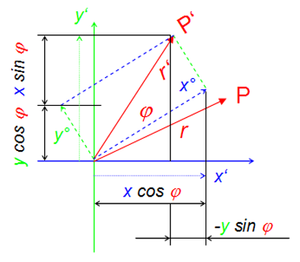
\includegraphics[width=0.4\textwidth]{drehung.png}
    \caption[http://systemdesign.ch/wiki/Drehung]{Drehung im $\mathbb{R}^2$}
    \label{fig:drehung}
\end{figure}~\\
Gegeben sei ein Punkt P $(x|y)$ in einem Koordinatensystem. Dieser Punkt soll um den Ursprung $(0|0)$ um den Winkel $\varphi$ gedreht werden.
\begin{center}
    \begin{tabular}{l l}
        P $(x|y)$ & $x = r * \sin(\alpha)$\\
        & $y = r * \cos(\alpha)$\\
        P' $(x'|y')$ & $x' = r * \sin(\alpha + \varphi)$\\
        & $y' = r * \cos(\alpha + \varphi)$
    \end{tabular}

    $$\downarrow$$

    \textbf{Additionstheorem}
    $$\sin(\alpha \pm \beta) = \sin(\alpha) * \cos(\beta) \pm \cos(\alpha) * \sin(\beta)$$
    $$\cos(\alpha \pm \beta) = \cos(\alpha) * \cos(\beta) \pm \sin(\alpha) * \sin(\beta)$$
    $$\downarrow$$
    \begin{tabular}{l l}
        P' $(x'|y')$ & $x' = r * \sin(\alpha) * \cos(\varphi) + r * \cos(\alpha) * \sin(\varphi)$\\
        & $y' = r * \cos(\alpha) * \cos(\varphi) - r * \sin(\alpha) * \sin(\varphi)$
    \end{tabular}
    $$\downarrow$$
    \begin{tabular}{l l}
        P' $(x'|y')$ & $x' = x * \cos(\varphi) + y * \sin(\varphi)$\\
        & $y' = y * \cos(\varphi) - x * \sin(\varphi)$
    \end{tabular}
    $$\downarrow$$
    $$P' \begin{pmatrix}x'\\y'\end{pmatrix} =
    D \begin{pmatrix}
        \cos(\varphi) & \sin(\varphi)\\
        -\sin(\varphi) & \cos(\varphi)
    \end{pmatrix} *
    P \begin{pmatrix}x\\y\end{pmatrix}
    $$
\end{center}

\newpage
\paragraph{Drehmatrix}~\\
Beschreibt eine Drehung um den Ursprung um den Winkel $\varphi$.
$$
D = \begin{pmatrix}
\cos(\varphi) & \sin(\varphi)\\
-\sin(\varphi) & \cos(\varphi)
\end{pmatrix}
$$

\paragraph{Spiegelungsmatrix}~\\
Beschreibt die Spiegelung an einer Geraden, durch den Ursprung mit der Steigung $\varphi$.
$$
Sp = \begin{pmatrix}
\cos(2\varphi) & \sin(2\varphi)\\
\sin(2\varphi) & -\cos(2\varphi)
\end{pmatrix}
$$
\paragraph{Streckungsmatrix}~\\
Beschreibt eine Streckung um $S_x$ in x-Richtung und um $S_y$ in y-Richtung.
$$
St = \begin{pmatrix}
S_x & 0\\
0 & S_y
\end{pmatrix}
$$

\subsubsection{Anwendung}
% \begin{figure}[hh]
%    \centering
%    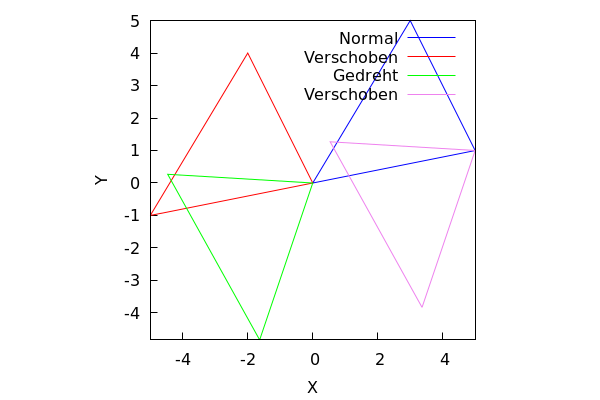
\includegraphics[width=0.6\textwidth]{dreieck.png}
% \end{figure}
\begin{enumerate}
    \item Verschieben des Ankerpunktes zum Ursprung. $$A' = A - \overrightarrow{OB}$$
    \item Matrix anwenden durch Multiplikation. $$A'' = D \cdot A \quad \quad A'' = Sp \cdot A \quad \quad A'' = St \cdot A$$
    \item Zurückschieben um den Ortsvektor des Ankerpunktes. $$A''' = A + \overrightarrow{OB}$$
\end{enumerate}

\printglossaries{}

\begin{thebibliography}{9}
    \bibitem{determinante} http://www.mathe-online.at/materialien/klaus.berger/files/Matrizen/determinante.pdf
    \bibitem{skalarprodukt} https://de.wikipedia.org/wiki/Skalarprodukt
\end{thebibliography}

\listoffigures

\end{document}
